\documentclass[12pt,a4paper]{article}
\usepackage[utf8]{inputenc}
\usepackage[spanish]{babel}
\usepackage{amsmath}
\usepackage{amsfonts}
\usepackage{amssymb}
\usepackage[left=2cm,right=2cm,top=2cm,bottom=2cm]{geometry}
\usepackage[T1]{fontenc}
\usepackage{titlesec}
\usepackage{hyperref}
\hypersetup{
    colorlinks=true,
    linkcolor=blue,
    urlcolor=red,
    pdftitle={Tarea 3 Viajero},
    }
\author{Lic. Arnoldo Del Toro Peña}
\title{Tarea: Algoritmo Set Covering}
\date{\today}
\usepackage{natbib}
\bibliographystyle{dinat}
\usepackage{graphicx}
\titleformat{\section}[display]
{\normalfont}{\filcenter\small
\ SECCIÓN \thesection   }
{0.5pt}{\Large\bfseries\filcenter  \hrulefill \\ }

%% %--
%\usepackage{titlesec}
%\titleformat{\section}[frame]{\normalfont} %
%{\filright\footnotesize\enspace SECCIÓN \thesection\enspace} %
%{8pt}{\Large\bfseries\filcenter} %
%%-




\begin{document}

\maketitle



\thispagestyle{empty}
\begin{abstract}
    Uso de un método metahurístico para la solución a un problema del viajero utilizando programación en python.
\end{abstract}
{\centering \textit{Palabras clave: python,viajero, metahurística.}}
\section{Introducción}
En este documento se presentarán los resultados a las instancias obtenidas, se compararán con los resultados óptimos que se presentan a continuación:

\begin{table}[h!]
\centering
\begin{tabular}{|c|c|c|c|c|}
\hline
\multicolumn{1}{|l|}{\textbf{Instancias de Prueba}} & \multicolumn{1}{l|}{\textit{Nombre de la instancia}}  & \multicolumn{1}{c|}{\textit{nodos}} & \textit{Óptimo} \\ \hline
\textit{76}                                          &  pr76.tsp                                & 76                            & 108159            \\ \hline
\textit{105}                                          & lin105.tsp                                 & 105                            & 14379             \\ \hline
\textit{280}                                          & a280.tsp                                 & 280                           & -            \\ \hline
\textit{130}                                          & ch130.tsp                                 & 130                            & 6110             \\ \hline
\textit{225}                                          & tsp225.tsp                                 & 225                            & 3919             \\ \hline

\end{tabular}
\end{table}

Más adelante analizaremos las diferencias entre estos resultados y los que obtuvimos.

\section{Descripción}
 El algoritmo que se pidió fue el del nodo más cercano el cual se menciona en el siguiente diagrama:
 \begin{figure}[ht]
    \centering
    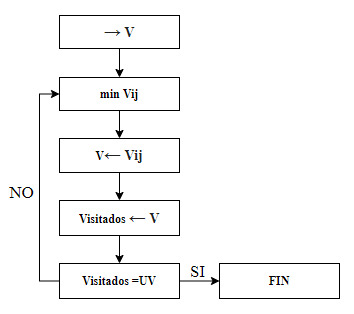
\includegraphics[scale = 0.5]{diagrama.jpeg}
    \caption{Diagrama}     
 \end{figure}
 \newpage Una breve explicación del digrama anterior; podemos observar que una vez que marcamos el nodo se exploran sus conexiones con nodos no marcados y se selecciona el menor y esto se repite hasta marcar todos los nodos.
\section{Descripción del algoritmo}
 El algoritmo se finaliza cuando todos los nodos estan marcados y tenemos que agregar el nodo inicial al final para poder cerrar el recorrido.Podemos enumerar sus pasos de la siguiente manera:
\begin{enumerate}
    \item Elección de un vértice arbitrario respecto al vértice actual.
    \item Descubra la arista de menor distancia que ya este conectada al vértice actual y a un vértice no visitado V.
    \item Convierta el vértice actual en V.
    \item Marque V como visitado.
    \item Si todos los vértices del dominio estuvieran visitados, cierre el algoritmo.
    \item Vaya al paso 2
\end{enumerate}
\section{Implementación} 
El algoritmo se programó en lenguaje python con referencias en \cite{van1991guia}, \cite{van2017tutorial} y \cite{chun2001core}, y se puede verificar en el siguiente repositorio de: \href{https://github.com/arnoldae9/PycharmProjects.git}{git-hub}.

\section{Resultados} 
Los resultados se pueden ver en el mismo enlace de git-hub, en los documentos txt, sin embargo se presentarán a continuación en una forma más ordenada:
\\ Los viajes los podemos encontrar en los archivos 76.txt, 105.txt, 280.txt, 130.txt, 225.txt disponibles en el repositorio de Git mencionado en la parte de arriba. 
\begin{table}[h!]
    \centering
    \resizebox*{15 cm}{!}{\begin{tabular}{|c|c|c|c|c|c|c|}
        \hline
        \multicolumn{1}{|l|}{\textbf{Instancias de Prueba}} & \multicolumn{1}{l|}{\textit{Nombre de la instancia}}  & \multicolumn{1}{c|}{\textit{nodos}} & \textit{Óptimo} & \textit{Aproximado} & \textit{error \%}       \\ \hline
        \textit{76}                                          &  pr76.tsp                                & 76                            & 108159                            & 137192.62           & 26.84 \%       \\ \hline
        \textit{105}                                          & lin105.tsp                                 & 105                            & 14379                         & 18383.53            & 27.89 \%      \\ \hline
        \textit{280}                                          & a280.tsp                                 & 280                           & -                 & 4227.54             &      \\ \hline
        \textit{130}                                          & ch130.tsp                                 & 130                            & 6110                           & 7318.21             & 19.77 \%     \\ \hline
        \textit{225}                                          & tsp225.tsp                                 & 225                            & 3919                          & 4991.92             & 27.37 \%     \\ \hline
        &&&& \bfseries{Promedio:} & 25.46 \%  \\ \hline
        \end{tabular}}
    \end{table}
\section{Mejoras}
La idea de seleccionar el nodo mas cercano al nodo actual depende totalmente del nodo inicial; una idea que tuve fue ir tomando como nodo inicial cada uno de los nodos del viaje, entonces al final tendremos varias soluciones de las cuales podemos tomar la mejor opción.
\section{Conclusiones} 
Si observamos los porcentajes, podemos decir que todos rondan el 20 \% aun así, personalmente 20 \% de error es demasiado alto, sin duda tenemos que buscar mejorar el algoritmo o buscar una opción mejor.
\newpage %#TODO comentario tipo todo
% #FIXME repara esto
\bibliography{biblio}
\end{document}
